\documentclass[10pt]{article}

\usepackage{amsfonts}
\usepackage{amsmath}
\usepackage{geometry}
\usepackage{xcolor,graphicx}
%\usepackage{wrapfig}
\usepackage{subcaption}
%\usepackage{hyperref}

\title{Simulating the Universe}
\author{Najla Alhamadi, Michael Cock, Rebecca Halloran, Brady Metherall, Hector Robinson}

\newgeometry{margin=1in}
\setlength\parindent{0pt}

\begin{document}
\maketitle

\begin{figure}[htbp]
\centering
% GNUPLOT: LaTeX picture with Postscript
\begingroup
  \makeatletter
  \providecommand\color[2][]{%
    \GenericError{(gnuplot) \space\space\space\@spaces}{%
      Package color not loaded in conjunction with
      terminal option `colourtext'%
    }{See the gnuplot documentation for explanation.%
    }{Either use 'blacktext' in gnuplot or load the package
      color.sty in LaTeX.}%
    \renewcommand\color[2][]{}%
  }%
  \providecommand\includegraphics[2][]{%
    \GenericError{(gnuplot) \space\space\space\@spaces}{%
      Package graphicx or graphics not loaded%
    }{See the gnuplot documentation for explanation.%
    }{The gnuplot epslatex terminal needs graphicx.sty or graphics.sty.}%
    \renewcommand\includegraphics[2][]{}%
  }%
  \providecommand\rotatebox[2]{#2}%
  \@ifundefined{ifGPcolor}{%
    \newif\ifGPcolor
    \GPcolorfalse
  }{}%
  \@ifundefined{ifGPblacktext}{%
    \newif\ifGPblacktext
    \GPblacktexttrue
  }{}%
  % define a \g@addto@macro without @ in the name:
  \let\gplgaddtomacro\g@addto@macro
  % define empty templates for all commands taking text:
  \gdef\gplbacktext{}%
  \gdef\gplfronttext{}%
  \makeatother
  \ifGPblacktext
    % no textcolor at all
    \def\colorrgb#1{}%
    \def\colorgray#1{}%
  \else
    % gray or color?
    \ifGPcolor
      \def\colorrgb#1{\color[rgb]{#1}}%
      \def\colorgray#1{\color[gray]{#1}}%
      \expandafter\def\csname LTw\endcsname{\color{white}}%
      \expandafter\def\csname LTb\endcsname{\color{black}}%
      \expandafter\def\csname LTa\endcsname{\color{black}}%
      \expandafter\def\csname LT0\endcsname{\color[rgb]{1,0,0}}%
      \expandafter\def\csname LT1\endcsname{\color[rgb]{0,1,0}}%
      \expandafter\def\csname LT2\endcsname{\color[rgb]{0,0,1}}%
      \expandafter\def\csname LT3\endcsname{\color[rgb]{1,0,1}}%
      \expandafter\def\csname LT4\endcsname{\color[rgb]{0,1,1}}%
      \expandafter\def\csname LT5\endcsname{\color[rgb]{1,1,0}}%
      \expandafter\def\csname LT6\endcsname{\color[rgb]{0,0,0}}%
      \expandafter\def\csname LT7\endcsname{\color[rgb]{1,0.3,0}}%
      \expandafter\def\csname LT8\endcsname{\color[rgb]{0.5,0.5,0.5}}%
    \else
      % gray
      \def\colorrgb#1{\color{black}}%
      \def\colorgray#1{\color[gray]{#1}}%
      \expandafter\def\csname LTw\endcsname{\color{white}}%
      \expandafter\def\csname LTb\endcsname{\color{black}}%
      \expandafter\def\csname LTa\endcsname{\color{black}}%
      \expandafter\def\csname LT0\endcsname{\color{black}}%
      \expandafter\def\csname LT1\endcsname{\color{black}}%
      \expandafter\def\csname LT2\endcsname{\color{black}}%
      \expandafter\def\csname LT3\endcsname{\color{black}}%
      \expandafter\def\csname LT4\endcsname{\color{black}}%
      \expandafter\def\csname LT5\endcsname{\color{black}}%
      \expandafter\def\csname LT6\endcsname{\color{black}}%
      \expandafter\def\csname LT7\endcsname{\color{black}}%
      \expandafter\def\csname LT8\endcsname{\color{black}}%
    \fi
  \fi
    \setlength{\unitlength}{0.0500bp}%
    \ifx\gptboxheight\undefined%
      \newlength{\gptboxheight}%
      \newlength{\gptboxwidth}%
      \newsavebox{\gptboxtext}%
    \fi%
    \setlength{\fboxrule}{0.5pt}%
    \setlength{\fboxsep}{1pt}%
\begin{picture}(7674.00,5760.00)%
    \gplgaddtomacro\gplbacktext{%
      \csname LTb\endcsname%
      \put(1003,1433){\makebox(0,0){\strut{}$0$}}%
      \put(1698,1294){\makebox(0,0){\strut{}$10$}}%
      \put(2392,1155){\makebox(0,0){\strut{}$20$}}%
      \put(3087,1015){\makebox(0,0){\strut{}$30$}}%
      \put(3782,876){\makebox(0,0){\strut{}$40$}}%
      \put(4476,737){\makebox(0,0){\strut{}$50$}}%
      \put(4685,794){\makebox(0,0){\strut{}$0$}}%
      \put(5086,1035){\makebox(0,0){\strut{}$10$}}%
      \put(5487,1276){\makebox(0,0){\strut{}$20$}}%
      \put(5888,1518){\makebox(0,0){\strut{}$30$}}%
      \put(6289,1759){\makebox(0,0){\strut{}$40$}}%
      \put(6690,2001){\makebox(0,0){\strut{}$50$}}%
      \put(972,1529){\makebox(0,0)[r]{\strut{}$0$}}%
      \put(972,2011){\makebox(0,0)[r]{\strut{}$10$}}%
      \put(972,2494){\makebox(0,0)[r]{\strut{}$20$}}%
      \put(972,2977){\makebox(0,0)[r]{\strut{}$30$}}%
      \put(972,3459){\makebox(0,0)[r]{\strut{}$40$}}%
      \put(972,3941){\makebox(0,0)[r]{\strut{}$50$}}%
      \put(174,2735){\makebox(0,0){\strut{}$z$}}%
    }%
    \gplgaddtomacro\gplfronttext{%
      \csname LTb\endcsname%
      \put(2333,879){\makebox(0,0){\strut{}$x$}}%
      \put(6442,1261){\makebox(0,0){\strut{}$y$}}%
      \put(174,2735){\makebox(0,0){\strut{}$z$}}%
      \put(7089,2580){\makebox(0,0)[l]{\strut{}$0$}}%
      \put(7089,2819){\makebox(0,0)[l]{\strut{}$1$}}%
      \put(7089,3058){\makebox(0,0)[l]{\strut{}$2$}}%
      \put(7089,3298){\makebox(0,0)[l]{\strut{}$3$}}%
      \put(7089,3537){\makebox(0,0)[l]{\strut{}$4$}}%
      \put(7089,3776){\makebox(0,0)[l]{\strut{}$5$}}%
      \put(7089,4016){\makebox(0,0)[l]{\strut{}$6$}}%
      \put(7089,4255){\makebox(0,0)[l]{\strut{}$7$}}%
      \put(7287,3477){\makebox(0,0){\strut{}$v$}}%
    }%
    \gplbacktext
    \put(0,0){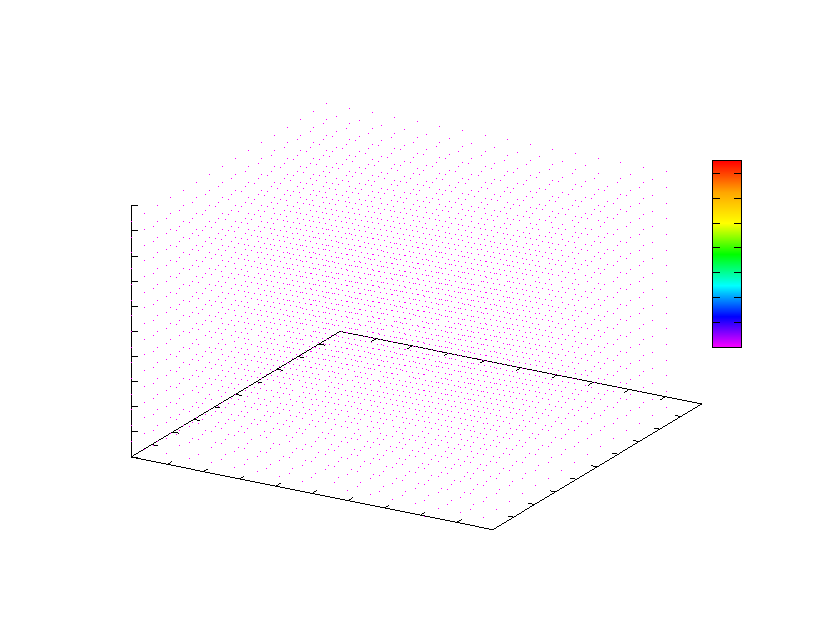
\includegraphics{Ordered}}%
    \gplfronttext
  \end{picture}%
\endgroup

\end{figure}

\begin{figure}[htbp]
\centering
\begin{subfigure}{\textwidth}
\centering
% GNUPLOT: LaTeX picture with Postscript
\begingroup
  \makeatletter
  \providecommand\color[2][]{%
    \GenericError{(gnuplot) \space\space\space\@spaces}{%
      Package color not loaded in conjunction with
      terminal option `colourtext'%
    }{See the gnuplot documentation for explanation.%
    }{Either use 'blacktext' in gnuplot or load the package
      color.sty in LaTeX.}%
    \renewcommand\color[2][]{}%
  }%
  \providecommand\includegraphics[2][]{%
    \GenericError{(gnuplot) \space\space\space\@spaces}{%
      Package graphicx or graphics not loaded%
    }{See the gnuplot documentation for explanation.%
    }{The gnuplot epslatex terminal needs graphicx.sty or graphics.sty.}%
    \renewcommand\includegraphics[2][]{}%
  }%
  \providecommand\rotatebox[2]{#2}%
  \@ifundefined{ifGPcolor}{%
    \newif\ifGPcolor
    \GPcolorfalse
  }{}%
  \@ifundefined{ifGPblacktext}{%
    \newif\ifGPblacktext
    \GPblacktexttrue
  }{}%
  % define a \g@addto@macro without @ in the name:
  \let\gplgaddtomacro\g@addto@macro
  % define empty templates for all commands taking text:
  \gdef\gplbacktext{}%
  \gdef\gplfronttext{}%
  \makeatother
  \ifGPblacktext
    % no textcolor at all
    \def\colorrgb#1{}%
    \def\colorgray#1{}%
  \else
    % gray or color?
    \ifGPcolor
      \def\colorrgb#1{\color[rgb]{#1}}%
      \def\colorgray#1{\color[gray]{#1}}%
      \expandafter\def\csname LTw\endcsname{\color{white}}%
      \expandafter\def\csname LTb\endcsname{\color{black}}%
      \expandafter\def\csname LTa\endcsname{\color{black}}%
      \expandafter\def\csname LT0\endcsname{\color[rgb]{1,0,0}}%
      \expandafter\def\csname LT1\endcsname{\color[rgb]{0,1,0}}%
      \expandafter\def\csname LT2\endcsname{\color[rgb]{0,0,1}}%
      \expandafter\def\csname LT3\endcsname{\color[rgb]{1,0,1}}%
      \expandafter\def\csname LT4\endcsname{\color[rgb]{0,1,1}}%
      \expandafter\def\csname LT5\endcsname{\color[rgb]{1,1,0}}%
      \expandafter\def\csname LT6\endcsname{\color[rgb]{0,0,0}}%
      \expandafter\def\csname LT7\endcsname{\color[rgb]{1,0.3,0}}%
      \expandafter\def\csname LT8\endcsname{\color[rgb]{0.5,0.5,0.5}}%
    \else
      % gray
      \def\colorrgb#1{\color{black}}%
      \def\colorgray#1{\color[gray]{#1}}%
      \expandafter\def\csname LTw\endcsname{\color{white}}%
      \expandafter\def\csname LTb\endcsname{\color{black}}%
      \expandafter\def\csname LTa\endcsname{\color{black}}%
      \expandafter\def\csname LT0\endcsname{\color{black}}%
      \expandafter\def\csname LT1\endcsname{\color{black}}%
      \expandafter\def\csname LT2\endcsname{\color{black}}%
      \expandafter\def\csname LT3\endcsname{\color{black}}%
      \expandafter\def\csname LT4\endcsname{\color{black}}%
      \expandafter\def\csname LT5\endcsname{\color{black}}%
      \expandafter\def\csname LT6\endcsname{\color{black}}%
      \expandafter\def\csname LT7\endcsname{\color{black}}%
      \expandafter\def\csname LT8\endcsname{\color{black}}%
    \fi
  \fi
    \setlength{\unitlength}{0.0500bp}%
    \ifx\gptboxheight\undefined%
      \newlength{\gptboxheight}%
      \newlength{\gptboxwidth}%
      \newsavebox{\gptboxtext}%
    \fi%
    \setlength{\fboxrule}{0.5pt}%
    \setlength{\fboxsep}{1pt}%
\begin{picture}(7674.00,5760.00)%
    \gplgaddtomacro\gplbacktext{%
      \csname LTb\endcsname%
      \put(990,704){\makebox(0,0)[r]{\strut{}$0$}}%
      \put(990,1662){\makebox(0,0)[r]{\strut{}$10$}}%
      \put(990,2620){\makebox(0,0)[r]{\strut{}$20$}}%
      \put(990,3579){\makebox(0,0)[r]{\strut{}$30$}}%
      \put(990,4537){\makebox(0,0)[r]{\strut{}$40$}}%
      \put(990,5495){\makebox(0,0)[r]{\strut{}$50$}}%
      \put(1122,484){\makebox(0,0){\strut{}$0$}}%
      \put(2080,484){\makebox(0,0){\strut{}$10$}}%
      \put(3038,484){\makebox(0,0){\strut{}$20$}}%
      \put(3997,484){\makebox(0,0){\strut{}$30$}}%
      \put(4955,484){\makebox(0,0){\strut{}$40$}}%
      \put(5913,484){\makebox(0,0){\strut{}$50$}}%
    }%
    \gplgaddtomacro\gplfronttext{%
      \csname LTb\endcsname%
      \put(484,3099){\rotatebox{-270}{\makebox(0,0){\strut{}$y$}}}%
      \put(3517,154){\makebox(0,0){\strut{}$x$}}%
      \csname LTb\endcsname%
      \put(6404,704){\makebox(0,0)[l]{\strut{}$0$}}%
      \put(6404,1342){\makebox(0,0)[l]{\strut{}$2$}}%
      \put(6404,1981){\makebox(0,0)[l]{\strut{}$4$}}%
      \put(6404,2620){\makebox(0,0)[l]{\strut{}$6$}}%
      \put(6404,3259){\makebox(0,0)[l]{\strut{}$8$}}%
      \put(6404,3898){\makebox(0,0)[l]{\strut{}$10$}}%
      \put(6404,4536){\makebox(0,0)[l]{\strut{}$12$}}%
      \put(6404,5175){\makebox(0,0)[l]{\strut{}$14$}}%
      \put(6734,3099){\makebox(0,0){\strut{}$v$}}%
    }%
    \gplbacktext
    \put(0,0){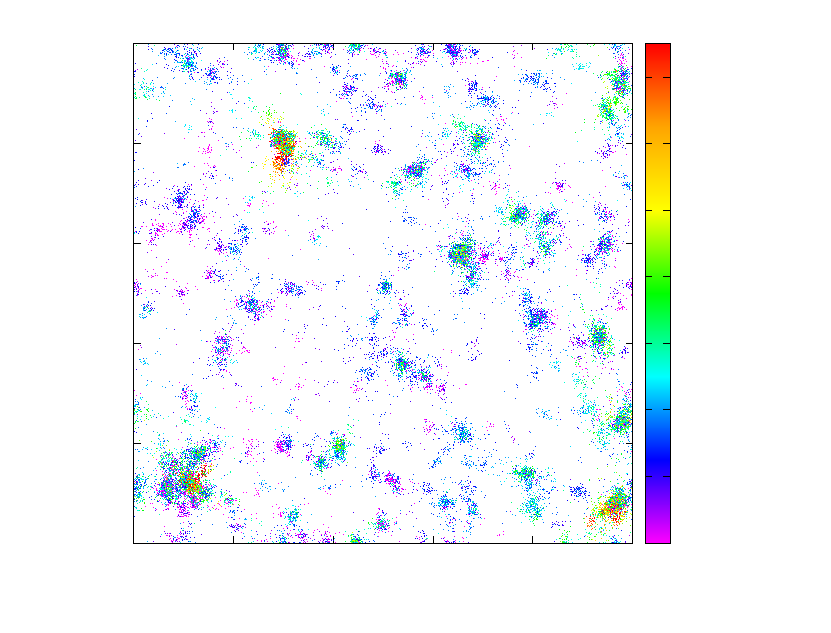
\includegraphics{Random2D}}%
    \gplfronttext
  \end{picture}%
\endgroup

\end{subfigure} \\
\begin{subfigure}{\textwidth}
\centering
% GNUPLOT: LaTeX picture with Postscript
\begingroup
  \makeatletter
  \providecommand\color[2][]{%
    \GenericError{(gnuplot) \space\space\space\@spaces}{%
      Package color not loaded in conjunction with
      terminal option `colourtext'%
    }{See the gnuplot documentation for explanation.%
    }{Either use 'blacktext' in gnuplot or load the package
      color.sty in LaTeX.}%
    \renewcommand\color[2][]{}%
  }%
  \providecommand\includegraphics[2][]{%
    \GenericError{(gnuplot) \space\space\space\@spaces}{%
      Package graphicx or graphics not loaded%
    }{See the gnuplot documentation for explanation.%
    }{The gnuplot epslatex terminal needs graphicx.sty or graphics.sty.}%
    \renewcommand\includegraphics[2][]{}%
  }%
  \providecommand\rotatebox[2]{#2}%
  \@ifundefined{ifGPcolor}{%
    \newif\ifGPcolor
    \GPcolorfalse
  }{}%
  \@ifundefined{ifGPblacktext}{%
    \newif\ifGPblacktext
    \GPblacktexttrue
  }{}%
  % define a \g@addto@macro without @ in the name:
  \let\gplgaddtomacro\g@addto@macro
  % define empty templates for all commands taking text:
  \gdef\gplbacktext{}%
  \gdef\gplfronttext{}%
  \makeatother
  \ifGPblacktext
    % no textcolor at all
    \def\colorrgb#1{}%
    \def\colorgray#1{}%
  \else
    % gray or color?
    \ifGPcolor
      \def\colorrgb#1{\color[rgb]{#1}}%
      \def\colorgray#1{\color[gray]{#1}}%
      \expandafter\def\csname LTw\endcsname{\color{white}}%
      \expandafter\def\csname LTb\endcsname{\color{black}}%
      \expandafter\def\csname LTa\endcsname{\color{black}}%
      \expandafter\def\csname LT0\endcsname{\color[rgb]{1,0,0}}%
      \expandafter\def\csname LT1\endcsname{\color[rgb]{0,1,0}}%
      \expandafter\def\csname LT2\endcsname{\color[rgb]{0,0,1}}%
      \expandafter\def\csname LT3\endcsname{\color[rgb]{1,0,1}}%
      \expandafter\def\csname LT4\endcsname{\color[rgb]{0,1,1}}%
      \expandafter\def\csname LT5\endcsname{\color[rgb]{1,1,0}}%
      \expandafter\def\csname LT6\endcsname{\color[rgb]{0,0,0}}%
      \expandafter\def\csname LT7\endcsname{\color[rgb]{1,0.3,0}}%
      \expandafter\def\csname LT8\endcsname{\color[rgb]{0.5,0.5,0.5}}%
    \else
      % gray
      \def\colorrgb#1{\color{black}}%
      \def\colorgray#1{\color[gray]{#1}}%
      \expandafter\def\csname LTw\endcsname{\color{white}}%
      \expandafter\def\csname LTb\endcsname{\color{black}}%
      \expandafter\def\csname LTa\endcsname{\color{black}}%
      \expandafter\def\csname LT0\endcsname{\color{black}}%
      \expandafter\def\csname LT1\endcsname{\color{black}}%
      \expandafter\def\csname LT2\endcsname{\color{black}}%
      \expandafter\def\csname LT3\endcsname{\color{black}}%
      \expandafter\def\csname LT4\endcsname{\color{black}}%
      \expandafter\def\csname LT5\endcsname{\color{black}}%
      \expandafter\def\csname LT6\endcsname{\color{black}}%
      \expandafter\def\csname LT7\endcsname{\color{black}}%
      \expandafter\def\csname LT8\endcsname{\color{black}}%
    \fi
  \fi
    \setlength{\unitlength}{0.0500bp}%
    \ifx\gptboxheight\undefined%
      \newlength{\gptboxheight}%
      \newlength{\gptboxwidth}%
      \newsavebox{\gptboxtext}%
    \fi%
    \setlength{\fboxrule}{0.5pt}%
    \setlength{\fboxsep}{1pt}%
\begin{picture}(7674.00,5760.00)%
    \gplgaddtomacro\gplbacktext{%
      \csname LTb\endcsname%
      \put(1003,1433){\makebox(0,0){\strut{}$0$}}%
      \put(1698,1294){\makebox(0,0){\strut{}$10$}}%
      \put(2392,1155){\makebox(0,0){\strut{}$20$}}%
      \put(3087,1015){\makebox(0,0){\strut{}$30$}}%
      \put(3782,876){\makebox(0,0){\strut{}$40$}}%
      \put(4476,737){\makebox(0,0){\strut{}$50$}}%
      \put(4685,794){\makebox(0,0){\strut{}$0$}}%
      \put(5086,1035){\makebox(0,0){\strut{}$10$}}%
      \put(5487,1276){\makebox(0,0){\strut{}$20$}}%
      \put(5888,1518){\makebox(0,0){\strut{}$30$}}%
      \put(6289,1759){\makebox(0,0){\strut{}$40$}}%
      \put(6690,2001){\makebox(0,0){\strut{}$50$}}%
      \put(972,1529){\makebox(0,0)[r]{\strut{}$0$}}%
      \put(972,2011){\makebox(0,0)[r]{\strut{}$10$}}%
      \put(972,2494){\makebox(0,0)[r]{\strut{}$20$}}%
      \put(972,2977){\makebox(0,0)[r]{\strut{}$30$}}%
      \put(972,3459){\makebox(0,0)[r]{\strut{}$40$}}%
      \put(972,3941){\makebox(0,0)[r]{\strut{}$50$}}%
      \put(174,2735){\makebox(0,0){\strut{}$z$}}%
    }%
    \gplgaddtomacro\gplfronttext{%
      \csname LTb\endcsname%
      \put(2333,879){\makebox(0,0){\strut{}$x$}}%
      \put(6442,1261){\makebox(0,0){\strut{}$y$}}%
      \put(174,2735){\makebox(0,0){\strut{}$z$}}%
      \put(7089,2580){\makebox(0,0)[l]{\strut{}$0$}}%
      \put(7089,2819){\makebox(0,0)[l]{\strut{}$2$}}%
      \put(7089,3058){\makebox(0,0)[l]{\strut{}$4$}}%
      \put(7089,3298){\makebox(0,0)[l]{\strut{}$6$}}%
      \put(7089,3537){\makebox(0,0)[l]{\strut{}$8$}}%
      \put(7089,3776){\makebox(0,0)[l]{\strut{}$10$}}%
      \put(7089,4016){\makebox(0,0)[l]{\strut{}$12$}}%
      \put(7089,4255){\makebox(0,0)[l]{\strut{}$14$}}%
      \put(7419,3477){\makebox(0,0){\strut{}$v$}}%
    }%
    \gplbacktext
    \put(0,0){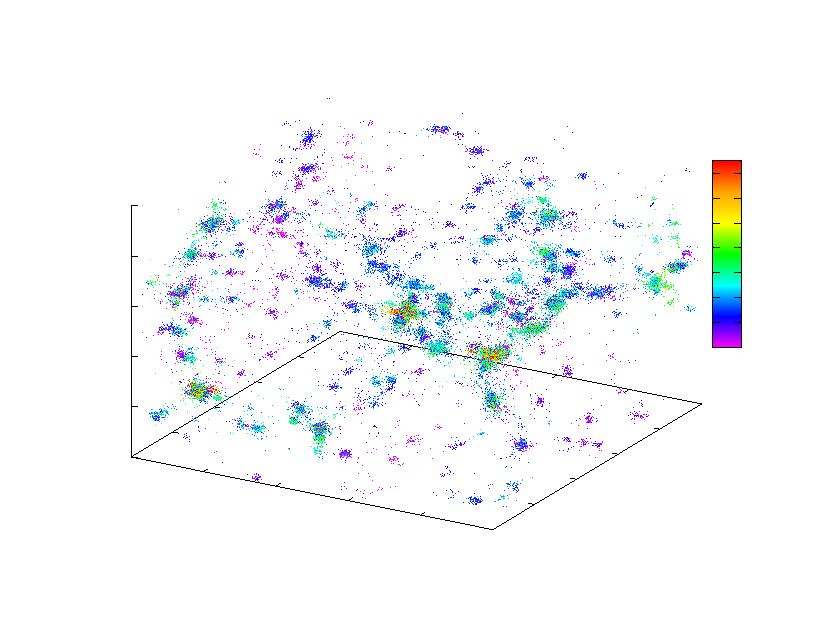
\includegraphics{Random3D}}%
    \gplfronttext
  \end{picture}%
\endgroup

\end{subfigure}
\end{figure}

\begin{figure}[htbp]
\centering
\begin{subfigure}{\textwidth}
\centering
% GNUPLOT: LaTeX picture with Postscript
\begingroup
  \makeatletter
  \providecommand\color[2][]{%
    \GenericError{(gnuplot) \space\space\space\@spaces}{%
      Package color not loaded in conjunction with
      terminal option `colourtext'%
    }{See the gnuplot documentation for explanation.%
    }{Either use 'blacktext' in gnuplot or load the package
      color.sty in LaTeX.}%
    \renewcommand\color[2][]{}%
  }%
  \providecommand\includegraphics[2][]{%
    \GenericError{(gnuplot) \space\space\space\@spaces}{%
      Package graphicx or graphics not loaded%
    }{See the gnuplot documentation for explanation.%
    }{The gnuplot epslatex terminal needs graphicx.sty or graphics.sty.}%
    \renewcommand\includegraphics[2][]{}%
  }%
  \providecommand\rotatebox[2]{#2}%
  \@ifundefined{ifGPcolor}{%
    \newif\ifGPcolor
    \GPcolorfalse
  }{}%
  \@ifundefined{ifGPblacktext}{%
    \newif\ifGPblacktext
    \GPblacktexttrue
  }{}%
  % define a \g@addto@macro without @ in the name:
  \let\gplgaddtomacro\g@addto@macro
  % define empty templates for all commands taking text:
  \gdef\gplbacktext{}%
  \gdef\gplfronttext{}%
  \makeatother
  \ifGPblacktext
    % no textcolor at all
    \def\colorrgb#1{}%
    \def\colorgray#1{}%
  \else
    % gray or color?
    \ifGPcolor
      \def\colorrgb#1{\color[rgb]{#1}}%
      \def\colorgray#1{\color[gray]{#1}}%
      \expandafter\def\csname LTw\endcsname{\color{white}}%
      \expandafter\def\csname LTb\endcsname{\color{black}}%
      \expandafter\def\csname LTa\endcsname{\color{black}}%
      \expandafter\def\csname LT0\endcsname{\color[rgb]{1,0,0}}%
      \expandafter\def\csname LT1\endcsname{\color[rgb]{0,1,0}}%
      \expandafter\def\csname LT2\endcsname{\color[rgb]{0,0,1}}%
      \expandafter\def\csname LT3\endcsname{\color[rgb]{1,0,1}}%
      \expandafter\def\csname LT4\endcsname{\color[rgb]{0,1,1}}%
      \expandafter\def\csname LT5\endcsname{\color[rgb]{1,1,0}}%
      \expandafter\def\csname LT6\endcsname{\color[rgb]{0,0,0}}%
      \expandafter\def\csname LT7\endcsname{\color[rgb]{1,0.3,0}}%
      \expandafter\def\csname LT8\endcsname{\color[rgb]{0.5,0.5,0.5}}%
    \else
      % gray
      \def\colorrgb#1{\color{black}}%
      \def\colorgray#1{\color[gray]{#1}}%
      \expandafter\def\csname LTw\endcsname{\color{white}}%
      \expandafter\def\csname LTb\endcsname{\color{black}}%
      \expandafter\def\csname LTa\endcsname{\color{black}}%
      \expandafter\def\csname LT0\endcsname{\color{black}}%
      \expandafter\def\csname LT1\endcsname{\color{black}}%
      \expandafter\def\csname LT2\endcsname{\color{black}}%
      \expandafter\def\csname LT3\endcsname{\color{black}}%
      \expandafter\def\csname LT4\endcsname{\color{black}}%
      \expandafter\def\csname LT5\endcsname{\color{black}}%
      \expandafter\def\csname LT6\endcsname{\color{black}}%
      \expandafter\def\csname LT7\endcsname{\color{black}}%
      \expandafter\def\csname LT8\endcsname{\color{black}}%
    \fi
  \fi
    \setlength{\unitlength}{0.0500bp}%
    \ifx\gptboxheight\undefined%
      \newlength{\gptboxheight}%
      \newlength{\gptboxwidth}%
      \newsavebox{\gptboxtext}%
    \fi%
    \setlength{\fboxrule}{0.5pt}%
    \setlength{\fboxsep}{1pt}%
\begin{picture}(7674.00,5760.00)%
    \gplgaddtomacro\gplbacktext{%
      \csname LTb\endcsname%
      \put(990,704){\makebox(0,0)[r]{\strut{}$0$}}%
      \put(990,1662){\makebox(0,0)[r]{\strut{}$10$}}%
      \put(990,2620){\makebox(0,0)[r]{\strut{}$20$}}%
      \put(990,3579){\makebox(0,0)[r]{\strut{}$30$}}%
      \put(990,4537){\makebox(0,0)[r]{\strut{}$40$}}%
      \put(990,5495){\makebox(0,0)[r]{\strut{}$50$}}%
      \put(1122,484){\makebox(0,0){\strut{}$0$}}%
      \put(2080,484){\makebox(0,0){\strut{}$10$}}%
      \put(3038,484){\makebox(0,0){\strut{}$20$}}%
      \put(3997,484){\makebox(0,0){\strut{}$30$}}%
      \put(4955,484){\makebox(0,0){\strut{}$40$}}%
      \put(5913,484){\makebox(0,0){\strut{}$50$}}%
    }%
    \gplgaddtomacro\gplfronttext{%
      \csname LTb\endcsname%
      \put(484,3099){\makebox(0,0){\strut{}$y$}}%
      \put(3517,154){\makebox(0,0){\strut{}$x$}}%
      \csname LTb\endcsname%
      \put(6404,704){\makebox(0,0)[l]{\strut{}$0$}}%
      \put(6404,1183){\makebox(0,0)[l]{\strut{}$5$}}%
      \put(6404,1662){\makebox(0,0)[l]{\strut{}$10$}}%
      \put(6404,2141){\makebox(0,0)[l]{\strut{}$15$}}%
      \put(6404,2620){\makebox(0,0)[l]{\strut{}$20$}}%
      \put(6404,3099){\makebox(0,0)[l]{\strut{}$25$}}%
      \put(6404,3578){\makebox(0,0)[l]{\strut{}$30$}}%
      \put(6404,4057){\makebox(0,0)[l]{\strut{}$35$}}%
      \put(6404,4536){\makebox(0,0)[l]{\strut{}$40$}}%
      \put(6404,5015){\makebox(0,0)[l]{\strut{}$45$}}%
      \put(6404,5495){\makebox(0,0)[l]{\strut{}$50$}}%
      \put(6734,3099){\makebox(0,0){\strut{}$z$}}%
    }%
    \gplbacktext
    \put(0,0){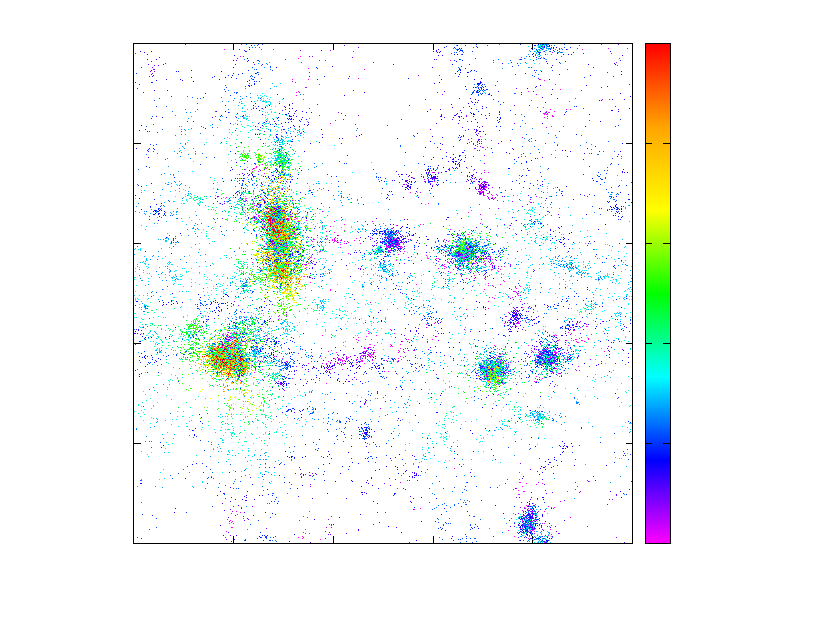
\includegraphics{Control}}%
    \gplfronttext
  \end{picture}%
\endgroup

\caption{Top-down view.}
\end{subfigure} \\
\begin{subfigure}{\textwidth}
\centering
% GNUPLOT: LaTeX picture with Postscript
\begingroup
  \makeatletter
  \providecommand\color[2][]{%
    \GenericError{(gnuplot) \space\space\space\@spaces}{%
      Package color not loaded in conjunction with
      terminal option `colourtext'%
    }{See the gnuplot documentation for explanation.%
    }{Either use 'blacktext' in gnuplot or load the package
      color.sty in LaTeX.}%
    \renewcommand\color[2][]{}%
  }%
  \providecommand\includegraphics[2][]{%
    \GenericError{(gnuplot) \space\space\space\@spaces}{%
      Package graphicx or graphics not loaded%
    }{See the gnuplot documentation for explanation.%
    }{The gnuplot epslatex terminal needs graphicx.sty or graphics.sty.}%
    \renewcommand\includegraphics[2][]{}%
  }%
  \providecommand\rotatebox[2]{#2}%
  \@ifundefined{ifGPcolor}{%
    \newif\ifGPcolor
    \GPcolorfalse
  }{}%
  \@ifundefined{ifGPblacktext}{%
    \newif\ifGPblacktext
    \GPblacktexttrue
  }{}%
  % define a \g@addto@macro without @ in the name:
  \let\gplgaddtomacro\g@addto@macro
  % define empty templates for all commands taking text:
  \gdef\gplbacktext{}%
  \gdef\gplfronttext{}%
  \makeatother
  \ifGPblacktext
    % no textcolor at all
    \def\colorrgb#1{}%
    \def\colorgray#1{}%
  \else
    % gray or color?
    \ifGPcolor
      \def\colorrgb#1{\color[rgb]{#1}}%
      \def\colorgray#1{\color[gray]{#1}}%
      \expandafter\def\csname LTw\endcsname{\color{white}}%
      \expandafter\def\csname LTb\endcsname{\color{black}}%
      \expandafter\def\csname LTa\endcsname{\color{black}}%
      \expandafter\def\csname LT0\endcsname{\color[rgb]{1,0,0}}%
      \expandafter\def\csname LT1\endcsname{\color[rgb]{0,1,0}}%
      \expandafter\def\csname LT2\endcsname{\color[rgb]{0,0,1}}%
      \expandafter\def\csname LT3\endcsname{\color[rgb]{1,0,1}}%
      \expandafter\def\csname LT4\endcsname{\color[rgb]{0,1,1}}%
      \expandafter\def\csname LT5\endcsname{\color[rgb]{1,1,0}}%
      \expandafter\def\csname LT6\endcsname{\color[rgb]{0,0,0}}%
      \expandafter\def\csname LT7\endcsname{\color[rgb]{1,0.3,0}}%
      \expandafter\def\csname LT8\endcsname{\color[rgb]{0.5,0.5,0.5}}%
    \else
      % gray
      \def\colorrgb#1{\color{black}}%
      \def\colorgray#1{\color[gray]{#1}}%
      \expandafter\def\csname LTw\endcsname{\color{white}}%
      \expandafter\def\csname LTb\endcsname{\color{black}}%
      \expandafter\def\csname LTa\endcsname{\color{black}}%
      \expandafter\def\csname LT0\endcsname{\color{black}}%
      \expandafter\def\csname LT1\endcsname{\color{black}}%
      \expandafter\def\csname LT2\endcsname{\color{black}}%
      \expandafter\def\csname LT3\endcsname{\color{black}}%
      \expandafter\def\csname LT4\endcsname{\color{black}}%
      \expandafter\def\csname LT5\endcsname{\color{black}}%
      \expandafter\def\csname LT6\endcsname{\color{black}}%
      \expandafter\def\csname LT7\endcsname{\color{black}}%
      \expandafter\def\csname LT8\endcsname{\color{black}}%
    \fi
  \fi
    \setlength{\unitlength}{0.0500bp}%
    \ifx\gptboxheight\undefined%
      \newlength{\gptboxheight}%
      \newlength{\gptboxwidth}%
      \newsavebox{\gptboxtext}%
    \fi%
    \setlength{\fboxrule}{0.5pt}%
    \setlength{\fboxsep}{1pt}%
\begin{picture}(7674.00,5760.00)%
    \gplgaddtomacro\gplbacktext{%
      \csname LTb\endcsname%
      \put(1003,1433){\makebox(0,0){\strut{}$0$}}%
      \put(1698,1294){\makebox(0,0){\strut{}$10$}}%
      \put(2392,1155){\makebox(0,0){\strut{}$20$}}%
      \put(3087,1015){\makebox(0,0){\strut{}$30$}}%
      \put(3782,876){\makebox(0,0){\strut{}$40$}}%
      \put(4476,737){\makebox(0,0){\strut{}$50$}}%
      \put(4685,794){\makebox(0,0){\strut{}$0$}}%
      \put(5086,1035){\makebox(0,0){\strut{}$10$}}%
      \put(5487,1276){\makebox(0,0){\strut{}$20$}}%
      \put(5888,1518){\makebox(0,0){\strut{}$30$}}%
      \put(6289,1759){\makebox(0,0){\strut{}$40$}}%
      \put(6690,2001){\makebox(0,0){\strut{}$50$}}%
      \put(972,1529){\makebox(0,0)[r]{\strut{}$0$}}%
      \put(972,2011){\makebox(0,0)[r]{\strut{}$10$}}%
      \put(972,2494){\makebox(0,0)[r]{\strut{}$20$}}%
      \put(972,2977){\makebox(0,0)[r]{\strut{}$30$}}%
      \put(972,3459){\makebox(0,0)[r]{\strut{}$40$}}%
      \put(972,3941){\makebox(0,0)[r]{\strut{}$50$}}%
    }%
    \gplgaddtomacro\gplfronttext{%
      \csname LTb\endcsname%
      \put(2333,879){\makebox(0,0){\strut{}$x$}}%
      \put(6442,1261){\makebox(0,0){\strut{}$y$}}%
      \put(7089,2580){\makebox(0,0)[l]{\strut{}$0$}}%
      \put(7089,2759){\makebox(0,0)[l]{\strut{}$5$}}%
      \put(7089,2939){\makebox(0,0)[l]{\strut{}$10$}}%
      \put(7089,3118){\makebox(0,0)[l]{\strut{}$15$}}%
      \put(7089,3298){\makebox(0,0)[l]{\strut{}$20$}}%
      \put(7089,3477){\makebox(0,0)[l]{\strut{}$25$}}%
      \put(7089,3657){\makebox(0,0)[l]{\strut{}$30$}}%
      \put(7089,3836){\makebox(0,0)[l]{\strut{}$35$}}%
      \put(7089,4016){\makebox(0,0)[l]{\strut{}$40$}}%
      \put(7089,4195){\makebox(0,0)[l]{\strut{}$45$}}%
      \put(7089,4375){\makebox(0,0)[l]{\strut{}$50$}}%
      \put(7419,3477){\makebox(0,0){\strut{}$z$}}%
    }%
    \gplbacktext
    \put(0,0){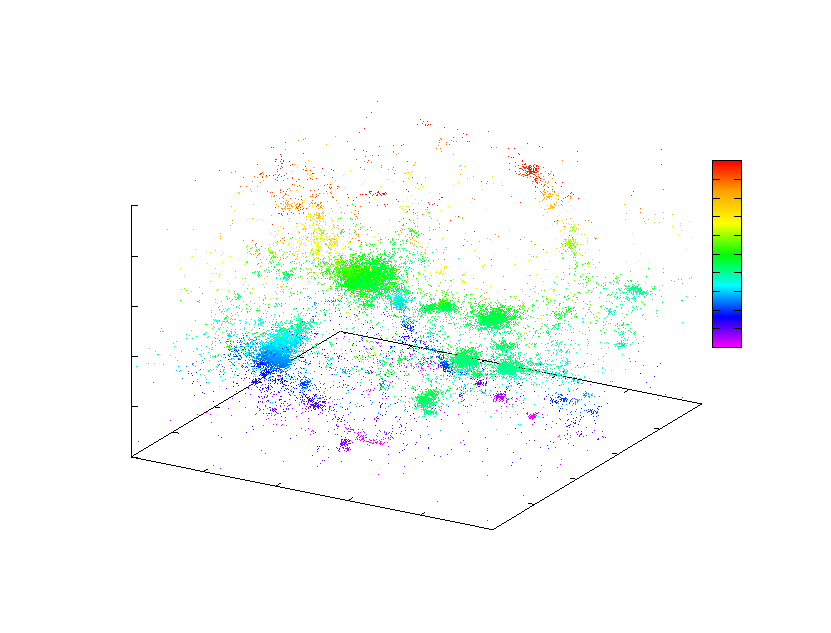
\includegraphics{Control3D}}%
    \gplfronttext
  \end{picture}%
\endgroup

\caption{3D view.}
\end{subfigure}
\caption{Control simulation.}
\end{figure}

\begin{figure}[htbp]
\centering
% GNUPLOT: LaTeX picture with Postscript
\begingroup
  \makeatletter
  \providecommand\color[2][]{%
    \GenericError{(gnuplot) \space\space\space\@spaces}{%
      Package color not loaded in conjunction with
      terminal option `colourtext'%
    }{See the gnuplot documentation for explanation.%
    }{Either use 'blacktext' in gnuplot or load the package
      color.sty in LaTeX.}%
    \renewcommand\color[2][]{}%
  }%
  \providecommand\includegraphics[2][]{%
    \GenericError{(gnuplot) \space\space\space\@spaces}{%
      Package graphicx or graphics not loaded%
    }{See the gnuplot documentation for explanation.%
    }{The gnuplot epslatex terminal needs graphicx.sty or graphics.sty.}%
    \renewcommand\includegraphics[2][]{}%
  }%
  \providecommand\rotatebox[2]{#2}%
  \@ifundefined{ifGPcolor}{%
    \newif\ifGPcolor
    \GPcolorfalse
  }{}%
  \@ifundefined{ifGPblacktext}{%
    \newif\ifGPblacktext
    \GPblacktexttrue
  }{}%
  % define a \g@addto@macro without @ in the name:
  \let\gplgaddtomacro\g@addto@macro
  % define empty templates for all commands taking text:
  \gdef\gplbacktext{}%
  \gdef\gplfronttext{}%
  \makeatother
  \ifGPblacktext
    % no textcolor at all
    \def\colorrgb#1{}%
    \def\colorgray#1{}%
  \else
    % gray or color?
    \ifGPcolor
      \def\colorrgb#1{\color[rgb]{#1}}%
      \def\colorgray#1{\color[gray]{#1}}%
      \expandafter\def\csname LTw\endcsname{\color{white}}%
      \expandafter\def\csname LTb\endcsname{\color{black}}%
      \expandafter\def\csname LTa\endcsname{\color{black}}%
      \expandafter\def\csname LT0\endcsname{\color[rgb]{1,0,0}}%
      \expandafter\def\csname LT1\endcsname{\color[rgb]{0,1,0}}%
      \expandafter\def\csname LT2\endcsname{\color[rgb]{0,0,1}}%
      \expandafter\def\csname LT3\endcsname{\color[rgb]{1,0,1}}%
      \expandafter\def\csname LT4\endcsname{\color[rgb]{0,1,1}}%
      \expandafter\def\csname LT5\endcsname{\color[rgb]{1,1,0}}%
      \expandafter\def\csname LT6\endcsname{\color[rgb]{0,0,0}}%
      \expandafter\def\csname LT7\endcsname{\color[rgb]{1,0.3,0}}%
      \expandafter\def\csname LT8\endcsname{\color[rgb]{0.5,0.5,0.5}}%
    \else
      % gray
      \def\colorrgb#1{\color{black}}%
      \def\colorgray#1{\color[gray]{#1}}%
      \expandafter\def\csname LTw\endcsname{\color{white}}%
      \expandafter\def\csname LTb\endcsname{\color{black}}%
      \expandafter\def\csname LTa\endcsname{\color{black}}%
      \expandafter\def\csname LT0\endcsname{\color{black}}%
      \expandafter\def\csname LT1\endcsname{\color{black}}%
      \expandafter\def\csname LT2\endcsname{\color{black}}%
      \expandafter\def\csname LT3\endcsname{\color{black}}%
      \expandafter\def\csname LT4\endcsname{\color{black}}%
      \expandafter\def\csname LT5\endcsname{\color{black}}%
      \expandafter\def\csname LT6\endcsname{\color{black}}%
      \expandafter\def\csname LT7\endcsname{\color{black}}%
      \expandafter\def\csname LT8\endcsname{\color{black}}%
    \fi
  \fi
    \setlength{\unitlength}{0.0500bp}%
    \ifx\gptboxheight\undefined%
      \newlength{\gptboxheight}%
      \newlength{\gptboxwidth}%
      \newsavebox{\gptboxtext}%
    \fi%
    \setlength{\fboxrule}{0.5pt}%
    \setlength{\fboxsep}{1pt}%
\begin{picture}(7674.00,5760.00)%
    \gplgaddtomacro\gplbacktext{%
      \csname LTb\endcsname%
      \put(814,704){\makebox(0,0)[r]{\strut{}$10$}}%
      \put(814,1236){\makebox(0,0)[r]{\strut{}$20$}}%
      \put(814,1769){\makebox(0,0)[r]{\strut{}$30$}}%
      \put(814,2301){\makebox(0,0)[r]{\strut{}$40$}}%
      \put(814,2833){\makebox(0,0)[r]{\strut{}$50$}}%
      \put(814,3366){\makebox(0,0)[r]{\strut{}$60$}}%
      \put(814,3898){\makebox(0,0)[r]{\strut{}$70$}}%
      \put(814,4430){\makebox(0,0)[r]{\strut{}$80$}}%
      \put(814,4963){\makebox(0,0)[r]{\strut{}$90$}}%
      \put(814,5495){\makebox(0,0)[r]{\strut{}$100$}}%
      \put(946,484){\makebox(0,0){\strut{}$0$}}%
      \put(2212,484){\makebox(0,0){\strut{}$0.2$}}%
      \put(3478,484){\makebox(0,0){\strut{}$0.4$}}%
      \put(4745,484){\makebox(0,0){\strut{}$0.6$}}%
      \put(6011,484){\makebox(0,0){\strut{}$0.8$}}%
      \put(7277,484){\makebox(0,0){\strut{}$1$}}%
    }%
    \gplgaddtomacro\gplfronttext{%
      \csname LTb\endcsname%
      \put(176,3099){\rotatebox{-270}{\makebox(0,0){\strut{}Average Acceleration}}}%
      \put(4111,154){\makebox(0,0){\strut{}$a$}}%
    }%
    \gplbacktext
    \put(0,0){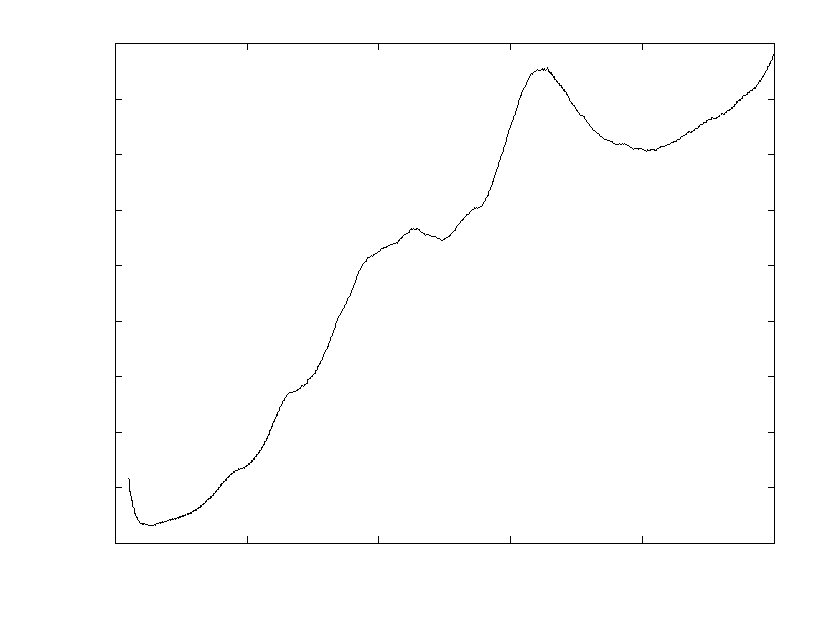
\includegraphics{Accel}}%
    \gplfronttext
  \end{picture}%
\endgroup

\end{figure}

\begin{figure}[htbp]
\centering
% GNUPLOT: LaTeX picture with Postscript
\begingroup
  \makeatletter
  \providecommand\color[2][]{%
    \GenericError{(gnuplot) \space\space\space\@spaces}{%
      Package color not loaded in conjunction with
      terminal option `colourtext'%
    }{See the gnuplot documentation for explanation.%
    }{Either use 'blacktext' in gnuplot or load the package
      color.sty in LaTeX.}%
    \renewcommand\color[2][]{}%
  }%
  \providecommand\includegraphics[2][]{%
    \GenericError{(gnuplot) \space\space\space\@spaces}{%
      Package graphicx or graphics not loaded%
    }{See the gnuplot documentation for explanation.%
    }{The gnuplot epslatex terminal needs graphicx.sty or graphics.sty.}%
    \renewcommand\includegraphics[2][]{}%
  }%
  \providecommand\rotatebox[2]{#2}%
  \@ifundefined{ifGPcolor}{%
    \newif\ifGPcolor
    \GPcolorfalse
  }{}%
  \@ifundefined{ifGPblacktext}{%
    \newif\ifGPblacktext
    \GPblacktexttrue
  }{}%
  % define a \g@addto@macro without @ in the name:
  \let\gplgaddtomacro\g@addto@macro
  % define empty templates for all commands taking text:
  \gdef\gplbacktext{}%
  \gdef\gplfronttext{}%
  \makeatother
  \ifGPblacktext
    % no textcolor at all
    \def\colorrgb#1{}%
    \def\colorgray#1{}%
  \else
    % gray or color?
    \ifGPcolor
      \def\colorrgb#1{\color[rgb]{#1}}%
      \def\colorgray#1{\color[gray]{#1}}%
      \expandafter\def\csname LTw\endcsname{\color{white}}%
      \expandafter\def\csname LTb\endcsname{\color{black}}%
      \expandafter\def\csname LTa\endcsname{\color{black}}%
      \expandafter\def\csname LT0\endcsname{\color[rgb]{1,0,0}}%
      \expandafter\def\csname LT1\endcsname{\color[rgb]{0,1,0}}%
      \expandafter\def\csname LT2\endcsname{\color[rgb]{0,0,1}}%
      \expandafter\def\csname LT3\endcsname{\color[rgb]{1,0,1}}%
      \expandafter\def\csname LT4\endcsname{\color[rgb]{0,1,1}}%
      \expandafter\def\csname LT5\endcsname{\color[rgb]{1,1,0}}%
      \expandafter\def\csname LT6\endcsname{\color[rgb]{0,0,0}}%
      \expandafter\def\csname LT7\endcsname{\color[rgb]{1,0.3,0}}%
      \expandafter\def\csname LT8\endcsname{\color[rgb]{0.5,0.5,0.5}}%
    \else
      % gray
      \def\colorrgb#1{\color{black}}%
      \def\colorgray#1{\color[gray]{#1}}%
      \expandafter\def\csname LTw\endcsname{\color{white}}%
      \expandafter\def\csname LTb\endcsname{\color{black}}%
      \expandafter\def\csname LTa\endcsname{\color{black}}%
      \expandafter\def\csname LT0\endcsname{\color{black}}%
      \expandafter\def\csname LT1\endcsname{\color{black}}%
      \expandafter\def\csname LT2\endcsname{\color{black}}%
      \expandafter\def\csname LT3\endcsname{\color{black}}%
      \expandafter\def\csname LT4\endcsname{\color{black}}%
      \expandafter\def\csname LT5\endcsname{\color{black}}%
      \expandafter\def\csname LT6\endcsname{\color{black}}%
      \expandafter\def\csname LT7\endcsname{\color{black}}%
      \expandafter\def\csname LT8\endcsname{\color{black}}%
    \fi
  \fi
    \setlength{\unitlength}{0.0500bp}%
    \ifx\gptboxheight\undefined%
      \newlength{\gptboxheight}%
      \newlength{\gptboxwidth}%
      \newsavebox{\gptboxtext}%
    \fi%
    \setlength{\fboxrule}{0.5pt}%
    \setlength{\fboxsep}{1pt}%
\begin{picture}(7674.00,5760.00)%
    \gplgaddtomacro\gplbacktext{%
      \csname LTb\endcsname%
      \put(1003,1433){\makebox(0,0){\strut{}$0$}}%
      \put(1698,1294){\makebox(0,0){\strut{}$10$}}%
      \put(2392,1155){\makebox(0,0){\strut{}$20$}}%
      \put(3087,1015){\makebox(0,0){\strut{}$30$}}%
      \put(3782,876){\makebox(0,0){\strut{}$40$}}%
      \put(4476,737){\makebox(0,0){\strut{}$50$}}%
      \put(4685,794){\makebox(0,0){\strut{}$0$}}%
      \put(5086,1035){\makebox(0,0){\strut{}$10$}}%
      \put(5487,1276){\makebox(0,0){\strut{}$20$}}%
      \put(5888,1518){\makebox(0,0){\strut{}$30$}}%
      \put(6289,1759){\makebox(0,0){\strut{}$40$}}%
      \put(6690,2001){\makebox(0,0){\strut{}$50$}}%
      \put(972,1529){\makebox(0,0)[r]{\strut{}$0$}}%
      \put(972,2011){\makebox(0,0)[r]{\strut{}$10$}}%
      \put(972,2494){\makebox(0,0)[r]{\strut{}$20$}}%
      \put(972,2977){\makebox(0,0)[r]{\strut{}$30$}}%
      \put(972,3459){\makebox(0,0)[r]{\strut{}$40$}}%
      \put(972,3941){\makebox(0,0)[r]{\strut{}$50$}}%
      \put(174,2735){\makebox(0,0){\strut{}$z$}}%
    }%
    \gplgaddtomacro\gplfronttext{%
      \csname LTb\endcsname%
      \put(2333,879){\makebox(0,0){\strut{}$x$}}%
      \put(6442,1261){\makebox(0,0){\strut{}$y$}}%
      \put(174,2735){\makebox(0,0){\strut{}$z$}}%
      \put(7089,2580){\makebox(0,0)[l]{\strut{}$0$}}%
      \put(7089,2939){\makebox(0,0)[l]{\strut{}$2$}}%
      \put(7089,3298){\makebox(0,0)[l]{\strut{}$4$}}%
      \put(7089,3657){\makebox(0,0)[l]{\strut{}$6$}}%
      \put(7089,4016){\makebox(0,0)[l]{\strut{}$8$}}%
      \put(7089,4375){\makebox(0,0)[l]{\strut{}$10$}}%
      \put(7419,3477){\makebox(0,0){\strut{}$v$}}%
    }%
    \gplbacktext
    \put(0,0){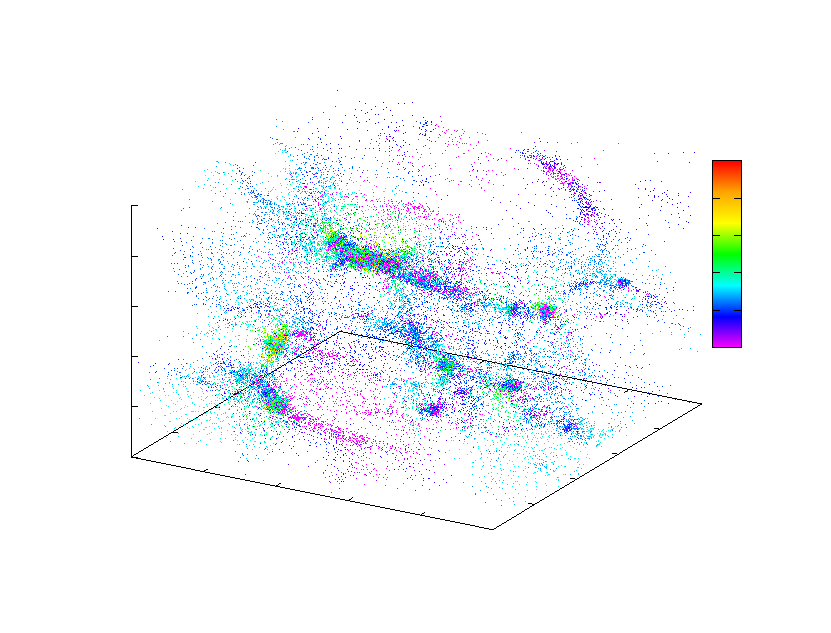
\includegraphics{1Ncells}}%
    \gplfronttext
  \end{picture}%
\endgroup

\caption{$N_c = n^{1/3}$}
\end{figure}

\begin{figure}[htbp]
\centering
% GNUPLOT: LaTeX picture with Postscript
\begingroup
  \makeatletter
  \providecommand\color[2][]{%
    \GenericError{(gnuplot) \space\space\space\@spaces}{%
      Package color not loaded in conjunction with
      terminal option `colourtext'%
    }{See the gnuplot documentation for explanation.%
    }{Either use 'blacktext' in gnuplot or load the package
      color.sty in LaTeX.}%
    \renewcommand\color[2][]{}%
  }%
  \providecommand\includegraphics[2][]{%
    \GenericError{(gnuplot) \space\space\space\@spaces}{%
      Package graphicx or graphics not loaded%
    }{See the gnuplot documentation for explanation.%
    }{The gnuplot epslatex terminal needs graphicx.sty or graphics.sty.}%
    \renewcommand\includegraphics[2][]{}%
  }%
  \providecommand\rotatebox[2]{#2}%
  \@ifundefined{ifGPcolor}{%
    \newif\ifGPcolor
    \GPcolorfalse
  }{}%
  \@ifundefined{ifGPblacktext}{%
    \newif\ifGPblacktext
    \GPblacktexttrue
  }{}%
  % define a \g@addto@macro without @ in the name:
  \let\gplgaddtomacro\g@addto@macro
  % define empty templates for all commands taking text:
  \gdef\gplbacktext{}%
  \gdef\gplfronttext{}%
  \makeatother
  \ifGPblacktext
    % no textcolor at all
    \def\colorrgb#1{}%
    \def\colorgray#1{}%
  \else
    % gray or color?
    \ifGPcolor
      \def\colorrgb#1{\color[rgb]{#1}}%
      \def\colorgray#1{\color[gray]{#1}}%
      \expandafter\def\csname LTw\endcsname{\color{white}}%
      \expandafter\def\csname LTb\endcsname{\color{black}}%
      \expandafter\def\csname LTa\endcsname{\color{black}}%
      \expandafter\def\csname LT0\endcsname{\color[rgb]{1,0,0}}%
      \expandafter\def\csname LT1\endcsname{\color[rgb]{0,1,0}}%
      \expandafter\def\csname LT2\endcsname{\color[rgb]{0,0,1}}%
      \expandafter\def\csname LT3\endcsname{\color[rgb]{1,0,1}}%
      \expandafter\def\csname LT4\endcsname{\color[rgb]{0,1,1}}%
      \expandafter\def\csname LT5\endcsname{\color[rgb]{1,1,0}}%
      \expandafter\def\csname LT6\endcsname{\color[rgb]{0,0,0}}%
      \expandafter\def\csname LT7\endcsname{\color[rgb]{1,0.3,0}}%
      \expandafter\def\csname LT8\endcsname{\color[rgb]{0.5,0.5,0.5}}%
    \else
      % gray
      \def\colorrgb#1{\color{black}}%
      \def\colorgray#1{\color[gray]{#1}}%
      \expandafter\def\csname LTw\endcsname{\color{white}}%
      \expandafter\def\csname LTb\endcsname{\color{black}}%
      \expandafter\def\csname LTa\endcsname{\color{black}}%
      \expandafter\def\csname LT0\endcsname{\color{black}}%
      \expandafter\def\csname LT1\endcsname{\color{black}}%
      \expandafter\def\csname LT2\endcsname{\color{black}}%
      \expandafter\def\csname LT3\endcsname{\color{black}}%
      \expandafter\def\csname LT4\endcsname{\color{black}}%
      \expandafter\def\csname LT5\endcsname{\color{black}}%
      \expandafter\def\csname LT6\endcsname{\color{black}}%
      \expandafter\def\csname LT7\endcsname{\color{black}}%
      \expandafter\def\csname LT8\endcsname{\color{black}}%
    \fi
  \fi
    \setlength{\unitlength}{0.0500bp}%
    \ifx\gptboxheight\undefined%
      \newlength{\gptboxheight}%
      \newlength{\gptboxwidth}%
      \newsavebox{\gptboxtext}%
    \fi%
    \setlength{\fboxrule}{0.5pt}%
    \setlength{\fboxsep}{1pt}%
\begin{picture}(7674.00,5760.00)%
    \gplgaddtomacro\gplbacktext{%
      \csname LTb\endcsname%
      \put(1003,1433){\makebox(0,0){\strut{}$0$}}%
      \put(1698,1294){\makebox(0,0){\strut{}$10$}}%
      \put(2392,1155){\makebox(0,0){\strut{}$20$}}%
      \put(3087,1015){\makebox(0,0){\strut{}$30$}}%
      \put(3782,876){\makebox(0,0){\strut{}$40$}}%
      \put(4476,737){\makebox(0,0){\strut{}$50$}}%
      \put(4685,794){\makebox(0,0){\strut{}$0$}}%
      \put(5086,1035){\makebox(0,0){\strut{}$10$}}%
      \put(5487,1276){\makebox(0,0){\strut{}$20$}}%
      \put(5888,1518){\makebox(0,0){\strut{}$30$}}%
      \put(6289,1759){\makebox(0,0){\strut{}$40$}}%
      \put(6690,2001){\makebox(0,0){\strut{}$50$}}%
      \put(972,1529){\makebox(0,0)[r]{\strut{}$0$}}%
      \put(972,2011){\makebox(0,0)[r]{\strut{}$10$}}%
      \put(972,2494){\makebox(0,0)[r]{\strut{}$20$}}%
      \put(972,2977){\makebox(0,0)[r]{\strut{}$30$}}%
      \put(972,3459){\makebox(0,0)[r]{\strut{}$40$}}%
      \put(972,3941){\makebox(0,0)[r]{\strut{}$50$}}%
      \put(174,2735){\makebox(0,0){\strut{}$z$}}%
    }%
    \gplgaddtomacro\gplfronttext{%
      \csname LTb\endcsname%
      \put(2333,879){\makebox(0,0){\strut{}$x$}}%
      \put(6442,1261){\makebox(0,0){\strut{}$y$}}%
      \put(174,2735){\makebox(0,0){\strut{}$z$}}%
      \put(7089,2580){\makebox(0,0)[l]{\strut{}$0$}}%
      \put(7089,2939){\makebox(0,0)[l]{\strut{}$20$}}%
      \put(7089,3298){\makebox(0,0)[l]{\strut{}$40$}}%
      \put(7089,3657){\makebox(0,0)[l]{\strut{}$60$}}%
      \put(7089,4016){\makebox(0,0)[l]{\strut{}$80$}}%
      \put(7089,4375){\makebox(0,0)[l]{\strut{}$100$}}%
      \put(7551,3477){\makebox(0,0){\strut{}$v$}}%
    }%
    \gplbacktext
    \put(0,0){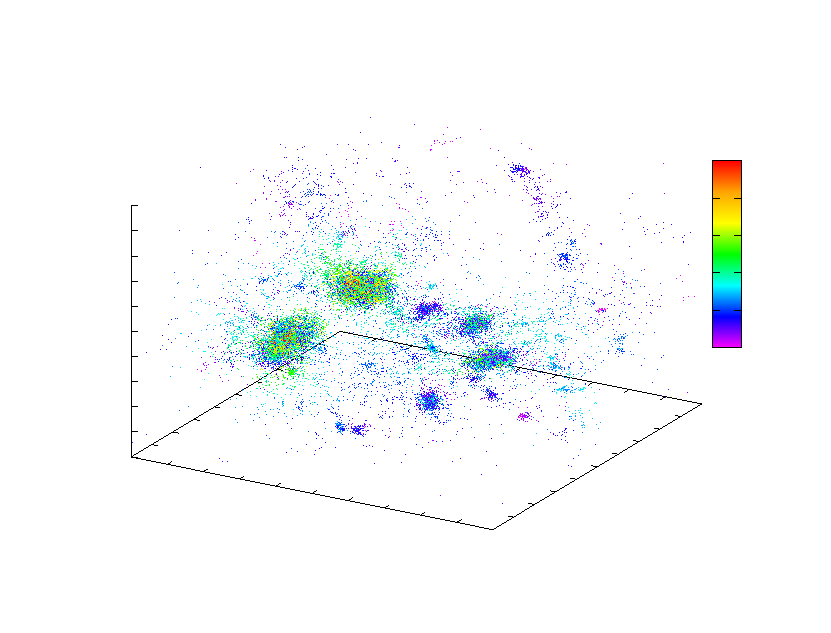
\includegraphics{3mass}}%
    \gplfronttext
  \end{picture}%
\endgroup

\caption{$\Omega_m = 3.0$, $\Omega_k = \Omega_\Lambda = 0$}
\end{figure}

\begin{figure}[htbp]
\centering
% GNUPLOT: LaTeX picture with Postscript
\begingroup
  \makeatletter
  \providecommand\color[2][]{%
    \GenericError{(gnuplot) \space\space\space\@spaces}{%
      Package color not loaded in conjunction with
      terminal option `colourtext'%
    }{See the gnuplot documentation for explanation.%
    }{Either use 'blacktext' in gnuplot or load the package
      color.sty in LaTeX.}%
    \renewcommand\color[2][]{}%
  }%
  \providecommand\includegraphics[2][]{%
    \GenericError{(gnuplot) \space\space\space\@spaces}{%
      Package graphicx or graphics not loaded%
    }{See the gnuplot documentation for explanation.%
    }{The gnuplot epslatex terminal needs graphicx.sty or graphics.sty.}%
    \renewcommand\includegraphics[2][]{}%
  }%
  \providecommand\rotatebox[2]{#2}%
  \@ifundefined{ifGPcolor}{%
    \newif\ifGPcolor
    \GPcolorfalse
  }{}%
  \@ifundefined{ifGPblacktext}{%
    \newif\ifGPblacktext
    \GPblacktexttrue
  }{}%
  % define a \g@addto@macro without @ in the name:
  \let\gplgaddtomacro\g@addto@macro
  % define empty templates for all commands taking text:
  \gdef\gplbacktext{}%
  \gdef\gplfronttext{}%
  \makeatother
  \ifGPblacktext
    % no textcolor at all
    \def\colorrgb#1{}%
    \def\colorgray#1{}%
  \else
    % gray or color?
    \ifGPcolor
      \def\colorrgb#1{\color[rgb]{#1}}%
      \def\colorgray#1{\color[gray]{#1}}%
      \expandafter\def\csname LTw\endcsname{\color{white}}%
      \expandafter\def\csname LTb\endcsname{\color{black}}%
      \expandafter\def\csname LTa\endcsname{\color{black}}%
      \expandafter\def\csname LT0\endcsname{\color[rgb]{1,0,0}}%
      \expandafter\def\csname LT1\endcsname{\color[rgb]{0,1,0}}%
      \expandafter\def\csname LT2\endcsname{\color[rgb]{0,0,1}}%
      \expandafter\def\csname LT3\endcsname{\color[rgb]{1,0,1}}%
      \expandafter\def\csname LT4\endcsname{\color[rgb]{0,1,1}}%
      \expandafter\def\csname LT5\endcsname{\color[rgb]{1,1,0}}%
      \expandafter\def\csname LT6\endcsname{\color[rgb]{0,0,0}}%
      \expandafter\def\csname LT7\endcsname{\color[rgb]{1,0.3,0}}%
      \expandafter\def\csname LT8\endcsname{\color[rgb]{0.5,0.5,0.5}}%
    \else
      % gray
      \def\colorrgb#1{\color{black}}%
      \def\colorgray#1{\color[gray]{#1}}%
      \expandafter\def\csname LTw\endcsname{\color{white}}%
      \expandafter\def\csname LTb\endcsname{\color{black}}%
      \expandafter\def\csname LTa\endcsname{\color{black}}%
      \expandafter\def\csname LT0\endcsname{\color{black}}%
      \expandafter\def\csname LT1\endcsname{\color{black}}%
      \expandafter\def\csname LT2\endcsname{\color{black}}%
      \expandafter\def\csname LT3\endcsname{\color{black}}%
      \expandafter\def\csname LT4\endcsname{\color{black}}%
      \expandafter\def\csname LT5\endcsname{\color{black}}%
      \expandafter\def\csname LT6\endcsname{\color{black}}%
      \expandafter\def\csname LT7\endcsname{\color{black}}%
      \expandafter\def\csname LT8\endcsname{\color{black}}%
    \fi
  \fi
    \setlength{\unitlength}{0.0500bp}%
    \ifx\gptboxheight\undefined%
      \newlength{\gptboxheight}%
      \newlength{\gptboxwidth}%
      \newsavebox{\gptboxtext}%
    \fi%
    \setlength{\fboxrule}{0.5pt}%
    \setlength{\fboxsep}{1pt}%
\begin{picture}(7674.00,5760.00)%
    \gplgaddtomacro\gplbacktext{%
      \csname LTb\endcsname%
      \put(1003,1433){\makebox(0,0){\strut{}$0$}}%
      \put(1698,1294){\makebox(0,0){\strut{}$10$}}%
      \put(2392,1155){\makebox(0,0){\strut{}$20$}}%
      \put(3087,1015){\makebox(0,0){\strut{}$30$}}%
      \put(3782,876){\makebox(0,0){\strut{}$40$}}%
      \put(4476,737){\makebox(0,0){\strut{}$50$}}%
      \put(4685,794){\makebox(0,0){\strut{}$0$}}%
      \put(5086,1035){\makebox(0,0){\strut{}$10$}}%
      \put(5487,1276){\makebox(0,0){\strut{}$20$}}%
      \put(5888,1518){\makebox(0,0){\strut{}$30$}}%
      \put(6289,1759){\makebox(0,0){\strut{}$40$}}%
      \put(6690,2001){\makebox(0,0){\strut{}$50$}}%
      \put(972,1529){\makebox(0,0)[r]{\strut{}$0$}}%
      \put(972,2011){\makebox(0,0)[r]{\strut{}$10$}}%
      \put(972,2494){\makebox(0,0)[r]{\strut{}$20$}}%
      \put(972,2977){\makebox(0,0)[r]{\strut{}$30$}}%
      \put(972,3459){\makebox(0,0)[r]{\strut{}$40$}}%
      \put(972,3941){\makebox(0,0)[r]{\strut{}$50$}}%
      \put(174,2735){\makebox(0,0){\strut{}$z$}}%
    }%
    \gplgaddtomacro\gplfronttext{%
      \csname LTb\endcsname%
      \put(2333,879){\makebox(0,0){\strut{}$x$}}%
      \put(6442,1261){\makebox(0,0){\strut{}$y$}}%
      \put(174,2735){\makebox(0,0){\strut{}$z$}}%
      \put(7089,2580){\makebox(0,0)[l]{\strut{}$0$}}%
      \put(7089,2939){\makebox(0,0)[l]{\strut{}$10$}}%
      \put(7089,3298){\makebox(0,0)[l]{\strut{}$20$}}%
      \put(7089,3657){\makebox(0,0)[l]{\strut{}$30$}}%
      \put(7089,4016){\makebox(0,0)[l]{\strut{}$40$}}%
      \put(7089,4375){\makebox(0,0)[l]{\strut{}$50$}}%
      \put(7419,3477){\makebox(0,0){\strut{}$v$}}%
    }%
    \gplbacktext
    \put(0,0){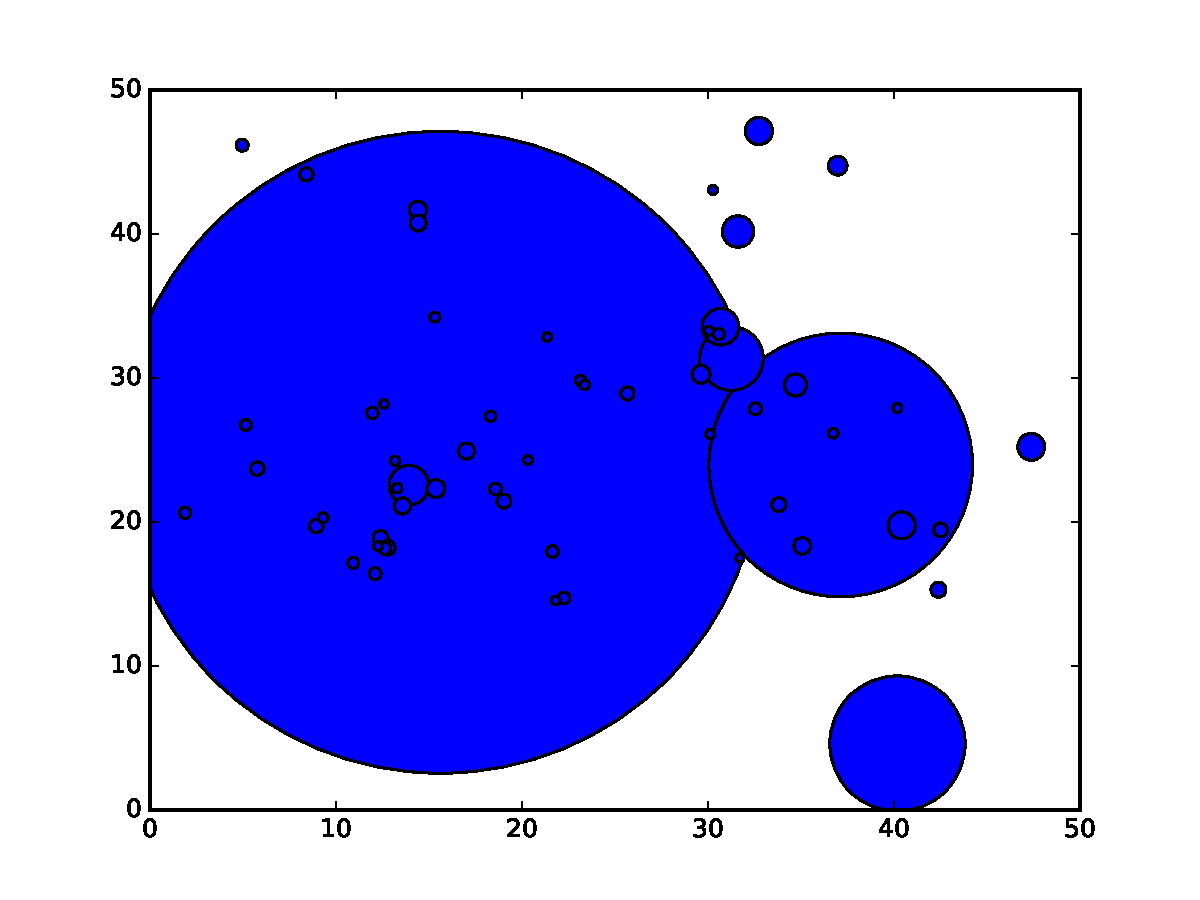
\includegraphics{N64}}%
    \gplfronttext
  \end{picture}%
\endgroup

\caption{$n = 64^3$}
\end{figure}

\end{document}
